%%%%%%%%%%%%%%%%%%%%%%%%%%%%%%%%%%%%%%%%%
% Template ini dibuat untuk makalah kolokium mahasiswa
% Program Alih Jenis (Ekstensi) Ilmu Komputer IPB
% Version 1.0 (18/05/2015)
%
% Template ini menggunakan template yang di-download dari:
% http://www.LaTeXTemplates.com
% Mathias Legrand (legrand.mathias@gmail.com)
% License: CC BY-NC-SA 3.0 (http://creativecommons.org/licenses/by-nc-sa/3.0/)
%
% Dimodifikasi untuk keperluan Program Studi
% Oleh: JULIO ADISANTOSO (julioipb@gmail.com)
%
% Untuk memudahkan penggunaan, maka diambil contoh makalah atas nama 
% Fithranto Faturakhman di bawah bimbingan Karlisa Priandana ILKOM-IPB.
% Silakan mengganti dan melengkapi file:
%    (1) kolokium_information.tex -- judul, nama, nim, email, pembimbing, dsb
%    (2) abstrak.tex -- abstrak makalah
%    (3) pendahuluan.tex -- berisi latar belakang, dsb
%    (4) metode.tex -- berisi metode penelitian
%    (5) daftar_pustaka.tex -- berisi daftar pustaka
%
%%%%%%%%%%%%%%%%%%%%%%%%%%%%%%%%%%%%%%%%%

%----------------------------------------------------------------------------------------
%	PACKAGES AND OTHER DOCUMENT CONFIGURATIONS
%----------------------------------------------------------------------------------------

\documentclass[fleqn,11pt]{SelfArx} % Document font size and equations flushed left
\usepackage[english]{babel}

%----------------------------------------------------------------------------------------
%	COLUMNS
%----------------------------------------------------------------------------------------

\setlength{\columnsep}{0.55cm} % Distance between the two columns of text
\setlength{\fboxrule}{0.75pt} % Width of the border around the abstract

%----------------------------------------------------------------------------------------
%	COLORS
%----------------------------------------------------------------------------------------

\definecolor{color1}{RGB}{0,0,90} % Color of the article title and sections
\definecolor{color2}{RGB}{0,20,20} % Color of the boxes behind the abstract and headings

%----------------------------------------------------------------------------------------
%	HYPERLINKS
%----------------------------------------------------------------------------------------

\usepackage{hyperref} % Required for hyperlinks
\hypersetup{hidelinks,colorlinks,breaklinks=true,urlcolor=color2,citecolor=color1,linkcolor=color1,bookmarksopen=false,pdftitle={Title},pdfauthor={Author}}


%
% Hyphenation untuk Indonesia 
%
% @author  Andreas Febrian
% @version 1.00
% 
% Tambahkan cara pemenggalan kata-kata yang salah dipenggal secara otomatis 
% oleh LaTeX. Jika kata tersebut dapat dipenggal dengan benar, maka tidak 
% perlu ditambahkan dalam berkas ini. Tanda pemenggalan kata menggunakan 
% tanda '-'; contoh: menarik  --> pemenggalan: me-na-rik
%

\hyphenation{
    % alphabhet A
    a-na-li-sa a-tur 
    a-pli-ka-si 
    % alphabhet B
    ba-ngun-an 
    be-be-ra-pa 
    ber-ge-rak
    ber-ke-lan-jut-an 
    ber-pe-nga-ruh 
    % alphabhet C
    ca-ri
    % alphabhet D
    di-sim-pan di-pim-pin de-ngan da-e-rah di-ba-ngun da-pat di-nya-ta-kan 
    di-sim-bol-kan di-pi-lih di-li-hat de-fi-ni-si
    % alphabhet E
    e-ner-gi eks-klu-sif
    % alphabhet F
    fa-si-li-tas
    % alphabhet G
    ga-bung-an ge-rak
    % alphabhet H
    ha-lang-an
    % alphabhet I
    % alphabhet J
    jang-krik
    % alphabhet K
    ke-hi-lang-an
    ku-ning 
    kua-li-tas ka-me-ra ke-mung-kin-an ke-se-pa-ham-an
    % alphabhet L
    ling-kung-an
    % alphabhet M
    me-neng-ah
    meng-a-tas-i me-mung-kin-kan me-nge-na-i me-ngi-rim-kan 
    meng-u-bah meng-a-dap-ta-si me-nya-ta-kan mo-di-fi-ka-si
    meng-a-tur meng-um-pul-kan
    % alphabhet N
    nya-ta non-eks-klu-sif
    % alphabhet O
    % alphabhet P
	pe-nye-rap-an 
	pe-ngon-trol
    pe-mo-del-an
    pe-ran  pe-ran-an-nya
    pem-ba-ngun-an pre-si-den pe-me-rin-tah prio-ri-tas peng-am-bil-an 
    peng-ga-bung-an pe-nga-was-an pe-ngem-bang-an 
    pe-nga-ruh pa-ra-lel-is-me per-hi-tung-an per-ma-sa-lah-an 
    pen-ca-ri-an peng-struk-tur-an
    pro-vin-si
    % alphabhet Q
    % alphabhet R
    ran-cang-an
    % alphabhet S
    si-mu-la-si sa-ngat
    % alphabhet T
    te-ngah
    ter-da-pat
    % alphabhet U
    % alphabhet V
    % alphabhet W
    % alphabhet X
    % alphabhet Y
    % alphabhet Z
    % special
}
% Tuliskan nama lengkap Anda
\def\namaMhs {Ferry Ramdhani}

% Tuliskan NIM Anda
\def\nim {G64134005}

% Tuliskan alamat email Anda
\def\emailMhs {ferry.ramdhani.16@gmail.com}

% Tuliskan nama lengkap dosen pembimbing
\def\namaDosen {Wisnu Ananta Kusuma}

% Tuliskan judul makalah kolokium di definisi "judul"
\def\judul {Implementasi Model Pemograman \textit{Map-Reduce} pada Pengelompokan Sekuen DNA dengan Metode \textit{Single Link}}

% Tuliskan kata kunci, dipisahkan oleh tanda titik-koma
\def\katakunci {\textit{k-mers frequency}; \textit{map-reduce}; sekuen DNA; \textit{single link}.}


\usepackage{xcolor,colortbl}
\usepackage{multicol}
\usepackage{multirow}
%\usepackage[urldate=iso8601, backend=biber, style=authoryear, url=true, doi=true, sorting=nyt]{biblatex}
\usepackage[urldate=iso8601,maxbibnames=9,maxcitenames=2,backend=biber,style=authoryear,url=true,doi=true,sorting=nyt]{biblatex}
\addbibresource{pustaka.bib}
\DefineBibliographyStrings{english}{%
	urlseen = {diunduh pada},
}
\renewbibmacro{in:}{\xspace dalam:}
\renewbibmacro*{volume+number+eid}{%
	\printfield{volume}%
	%  \setunit*{\adddot}% DELETED
	\setunit*{\addnbspace}% NEW (optional); there's also \addnbthinspace
	\printfield{number}%
	\setunit{\addcomma\space}%
	\printfield{eid}}
\DeclareFieldFormat[article]{number}{\mkbibparens{#1}}

%----------------------------------------------------------------------------------------
%	ARTICLE INFORMATION
%----------------------------------------------------------------------------------------

\JournalInfo{Makalah Kolokium Program S1 Ilmu Komputer Alih Jenis} % Journal information
\Archive{Departemen Ilmu Komputer, FMIPA-IPB} % Departemen ILKOM-IPB

\PaperTitle{\judul} 

\Authors{\namaMhs (\nim)*, \namaDosen} % Penulis
\affiliation{*\scriptsize\textbf{Alamat Email}: \emailMhs \normalsize} % Corresponding author

\Keywords{\scriptsize \katakunci \normalsize} 
\newcommand{\keywordname}{Kata Kunci} % Defines the keywords heading name

%----------------------------------------------------------------------------------------
%	ABSTRACT
%----------------------------------------------------------------------------------------
\Abstract{\scriptsize 
% ---- Tuliskan abstrak di bagian ini seperti contoh.
Indonesia mengalami kebakaran hutan yang signifikan. Pada tahun 2013 \textit{World Resources Institute} (WRI)  meneliti tren historis titik panas di Pulau Sumatera menggunakan data titik panas aktif \textit{National Aeronautics and Space Administration} (NASA). Pada 13-30 Juni 2013 terjadi 2643 total jumlah peringatan titik panas. Tahun berikutnya Pada  20 Februari hingga 11 Maret tahun 2014  titik panas meningkat menjadi 3101 peringatan titik panas. Salah satu upaya untuk menangani kebakaran hutan ialah dengan menganalisis data titik panas yaitu dengan menganalisis pencilan titik panas sehingga dapat diidentifikasi wilayah yang beresiko terjadinya kebakaran hutan. Beberapa penelitian terkait deteksi pencilan yang sudah dilakukan diantaranya menggunakan algoritme \textit{clustering} k-means dan juga menggunakan algoritme \textit{clustering} berbasis medoids. Kedua penelitian tersebut mendeteksi pencilan berdasarkan frekuensi terjadinya titik panas dan belum mendeteksi pencilan berdasarkan kepadatan penyebaran titik panas. Algoritme yang dapat mendeteksi pencilan berdasarkan kepadatan penyebaran titik panas ialah algoritme \textit{local outlier factor}.  Dengan algoritme \textit{local outlier factor} informasi mengenai wilayah yang berpotensi terjadi kebakaran hutan berdasarkan kepadatan penyebaran titik panas dapat dideteksi sehingga menjadi informasi tambahan untuk pengambilan keputusan oleh pihak terkait.
% ---- Akhir bagian abstrak
\normalsize}


%----------------------------------------------------------------------------------------

\begin{document}

\flushbottom % Makes all text pages the same height

\maketitle % Print the title and abstract box

\thispagestyle{empty} % Removes page numbering from the first page

%----------------------------------------------------------------------------------------
%	BAGIAN PENDAHULUAN
%----------------------------------------------------------------------------------------

%----------------------------------------------------------------------------------------
%	PENDAHULUAN
%----------------------------------------------------------------------------------------
\section*{PENDAHULUAN} % Sub Judul PENDAHULUAN
% Tuliskan isi Pendahuluan di bagian bawah ini. 
% Jika ingin menambahkan Sub-Sub Judul lainnya, silakan melihat contoh yang ada.
% Sub-sub Judul 
\subsection*{Latar Belakang}
Bioinformatika merupakan salah satu cabang ilmu yang memiliki peranan penting dalam kemajuan ilmu biologi, salah satunya adalah analisis sekuen \textit{deoxyribo nucleid acid} (DNA). DNA merupakan pembawa informasi genetik dari makhluk hidup. DNA merupakan rantai ganda dari nukleotida yang diikat dalam struktur \textit{helix} dikenal dengan \textit{double helix}.  Terdapat 4 basa utama dalam setiap nukleotida yaitu: \textit{adenine} (A), \textit{cytosin} (C), \textit{thymine} (T), dan \textit{guanine} (G).

Sekuen DNA didapatkan dengan memotong DNA dari suatu organisme yang diuraikan dan dipotong-potong menjadi \textit{reads}. \textit{Reads} tersebut berisi urutan huruf-huruf yang mewakili struktur primer dari molekul DNA. Sekuen DNA dalam bentuk \textit{file} akan disimpan dalam format FASTA. Dari \textit{reads} tersebut, dapat dilihat kode genetik setiap makhluk hidup. Variasi urutan basa setiap makhluk hidup memiliki kemiripan. Oleh karena itu, untuk mengetahui kekerabatan antarspesies diperlukan pengelompokan berdasarkan kesamaan ciri fiturnya.

Proses \textit{binning} pada sekuen DNA akan dilakukan untuk dikelompokan. Proses \textit{binning} dapat dilakukan dengan menggunakan metode \textit{unsupervised}, yaitu dengan pengelompokan. Pengelompokan adalah proses pembelajaran \textit{unsupervised} terhadap suatu pattern untuk dijadikan beberapa kelompok berdasarkan kemiripan (\citeauthor{JAIN1999} \cite*{JAIN1999}). Teknik pengelompokan digunakan untuk melihat kemiripan dengan melihat hasil dendogram dengan menggunakan metode hierarki. Metode hierarki juga dibagi menjadi beberapa macam seperti: \textit{single linkage}, \textit{complete linkage}, \textit{average linkage},  dan \textit{average group linkage}. Penelitian tentang \textit{single link} pada sekuens DNA pernah dilakukan oleh \citeauthor{TAMSIN2013} (\cite*{TAMSIN2013}). Pada penelitian tersebut, ekstraksi ciri yang digunakan adalah \textit{feature vector} dan tingkat kemiripan menggunakan \textit{cosine similarity}. Dari 8 studi kasus yang masing-masing terdiri dari 5 percobaan menggunakan 50 data sekuen DNA, didapatkan akurasi rata-rata 86.7$\%$ dengan nilai akurasi tertinggi 100$\%$ dan terendah 70$\%$. 

Sekuen DNA merupakan yang data yang sangat besar yang bahkan dapat mencapai ratusan megabase data (\citeauthor{KUNIN2008} \cite*{KUNIN2008}). Salah satu solusi untuk mengatasi hal tersebut adalah pemodelan \textit{map-reduce}. \textit{Map-reduce} merupakan model pemrograman yang penerapannya digunakan untuk memproses data yang berukuran besar  (\citeauthor{DEAN2004} \cite*{DEAN2004}). \textit{Map-reduce} diimplementasikan dalam \textit{platform} hadoop. Hadoop adalah \textit{framework} yang menangani data berskala besar dan digunakan untuk kluster pada Linux dengan tujuan untuk analisis data (\citeauthor{TAYLOR2010} \cite*{TAYLOR2010}).  Selain itu, penelitian terkait juga pernah dilakukan oleh \citeauthor{RASHEED2013} (\cite*{RASHEED2013}) yang menggunakan teknik pengelompokan dengan metode MC-MinH. Penelitian yang dilakukan berfokus pada evaluasi pengelompokan dan waktu komputasi. Hasilnya, sekuen hasil pengelompokan sama dengan sekuen yang ada pada metagenom.

Pada penelitian ini, penulis akan mengimplementasikan \textit{hierachical clustering} yang sama dengan yang dilakukan oleh \citeauthor{TAMSIN2013} (\cite*{TAMSIN2013}) dengan menggunakan \textit{single link} dengan \textit{k-mers} sebagai ekstrasi ciri. Namun, penulis akan menggunakan Hadoop dengan pemodelan \textit{map-reduce}. Dalam penelitian, ini juga ingin dilihat evalusi dari hasil pengelompokan dan waktu komputasi.

% Sub-sub perumusan masalah
\subsection*{Perumusan Masalah}
Perumasan masalah pada penelitian ini adalah penerapan \textit{map-reduce} untuk pengelompokan sekuen DNA dengan menggunakan metode \textit{single link}. Hasil dari pengelompokan akan dihitung waktu komputasinya.

% Sub-sub Judul 
\subsection*{Tujuan}
Tujuan dari penelitian ini adalah untuk mengimplementasikan pemodelan \textit{map-reduce} untuk pengelompokan sekuen DNA dengan \textit{single link}, melihat hasil pengelompokan sekuen DNA dan mengevaluasi hasil pengelompokan dengan metode \textit{single link} dan waktu komputasi

\subsection*{Ruang Lingkup}
Ruang lingkup penelitian adalah:
\begin{enumerate}[noitemsep] 
\item Penelitian ini menitik beratkan pada tahap pengelompokan.
\item Data sekuen DNA yang digunakan dengan format FASTA.
\item Data sekuen yang digunakan adalah DNA bakteri \textit{complete sequence}.
\item Data hasil simulasi bersifat bebas \textit{error}.
\item Bahasa pemrograman yang digunakan adalah Java.
\end{enumerate}

\subsection*{Manfaat}
Manfaat dari penelitian ini adalah sebagai pertimbangan untuk penerapan teknik pengelompokan dengan pemodelan \textit{map-reduce} pada sekuen DNA.

%----------------------------------------------------------------------------------------
%	PENDAHULUAN
%----------------------------------------------------------------------------------------
\section*{TINJAUAN PUSTAKA} % Sub Judul PENDAHULUAN
% Tuliskan isi Pendahuluan di bagian bawah ini. 
% Jika ingin menambahkan Sub-Sub Judul lainnya, silakan melihat contoh yang ada.
% Sub-sub Judul 
\subsection*{\textit{Map-reduce}}
\textit{Map-reduce} merupakan pemodelan pemograman yang digunakan untuk memproses data yang berukuran besar pada lingkungan paralel (\citeauthor{DEAN2004} \cite*{DEAN2004}). Pemodelan \textit{map-reduce} mempunyai \textit{run time system} yang menjadi salah satu kelebihan dari pemodelan ini. \textit{Run time system} dapat menangani masalah pembagian data dan penanganan kesalahan sistem. \textit{Map-reduce} memiliki dua tahap yang yaitu \textit{map} dan \textit{reduce}. \textit{Map} dan \textit{reduce} dijalankan secara terpisah namun sama-sama dilakukan secara paralel. Setiap langkah mempunyai atribut \textit{key} dan \textit{value} yang sepasang. \textit{Map} berfungsi untuk memetakan input ke dalam beberapa node dan memasangkan \textit{key} dan \textit{value} pada tiap node.  Komputer yang menjalankan tahap ini disebut \textit{mappers}. \textit{Reduce} berfungsi untuk menyatukan hasil dari \textit{map} dengan melihat \textit{key} yang diberikan pada tahap \textit{map}. \textit{Reduce} juga akan memblokir proses sampai data dari \textit{map} sudah semua ditransfer (\citeauthor{TAYLOR2010} \cite*{TAYLOR2010}). Komputer yang menjalankan tahap ini disebut \textit{reducers}.

% Sub-sub Judul 
\subsection*{\textit{K-mers Frequency}}
K-mers frequency merupakan frekuensi untuk menghitung banyaknya kemunculan dari subsequence yang mungkin dari 4 kombinasi (A, T, G, dan C) dengan panjang k pada suatu sekuen DNA. Setiap kombinasi akan dihitung sesuai dengan kombinasi dari sekuen DNA sebanyak k. Subsequence yang akan dihitung menggunakan nilai k sama dengan 3 akan menghasilkan pola ciri sebesar 43 atau 64 base pair. Pola ciri yang didapatkan adalah {AAA, AAC, AAT, AAG, ACA, ACC, ACT, ACG, ATA, ATC, ATT, ATG, AGA, AGC, AGT, AGG, CAA, CAC, CAT, CAG, CCA, CCC, CCT, CCG, CTA, CTC, CTT, CTG, CGA, CGC, CGT, CGG, TAA, TAC, TAT, TAG, TCA, TCC, TCT, TCG, TTA, TTC, TTT, TTG, TGA, TGC, TGT, TGG, GAA, GAC, GAT, GAG, GCA, GCC, GCT, GCG, GTA, GTC, GTT, GTG, GGA, GGC, GGT, GGG}. Ilustrasi perhitungan k-mers frequency  pada sekuen DNA dapat dilihat pada Gambar \ref{fig:mers}.

\begin{figure}[h!]\centering % Gunakan \begin{figure*} untuk memasukkan Gambar
	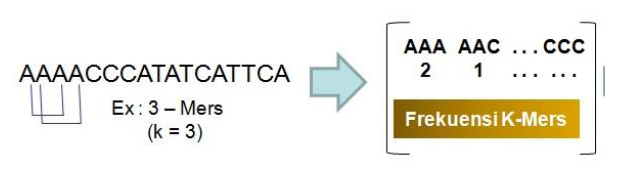
\includegraphics[width=200pt]{mers.png}
	\caption{Ilustrasi perhitungan \textit{k-mers}}
	\label{fig:mers}
\end{figure}

\subsection*{\textit{Single Link}}
Dalam analisis kluster pada dasarnya akan dilakukan pengelompokan secara alami terhadap sekelompok objek, dengan melakukan perbandingan terhadap masing-masing objek yang memiliki tingkat kesamaan atau jarak. Pengelompokan adalah proses pembelajaran \textit{unsupervised} terhadap suatu \textit{pattern} untuk dijadikan beberapa kelompok berdasarkan kemiripan (\citeauthor{JAIN1999} \cite*{JAIN1999}). Kluster adalah koleksi dari \textit{record} yang mirip dan tidak mirip dengan \textit{record} dari kluster lain. Pengelompokan  berbeda dengan klasifikasi, dalam hal ini tidak ada variabel target untuk dikelompokkan. Pengelompokan tidak mengklasifikasikan, meramalkan atau memprediksi nilai dari sebuah variabel target. Algoritme pengelompokan digunakan untuk menentukan segmen keseluruhan himpunan data menjadi subgrup yang relatif sama atau kluster, dengan kesamaan record dalam kluster dimaksimumkan dan kesamaan \textit{record} di luar kluster diminimumkan (\citeauthor{LAROSE2005} \cite*{LAROSE2005}).

Pengelompokan data dengan metode \textit{single link} termasuk ke dalam metode \textit{hierarchical agglomerative clustering}. \textit{Hierarchical} melihat objek yang mirip yang nantinya akan dikelompokkan. Hasilnya dalam bentuk dendogram yang akan menampilkan gambaran antarkelompok yang terdekat. Ilustrasi dendogram dapat dilihat pada Gambar \ref{fig:dendogram}.

\begin{figure}[h!] % Gunakan \begin{figure*} untuk memasukkan Gambar
	\centering
	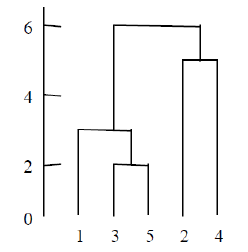
\includegraphics[width=200pt]{den.png}
	\caption{Ilustrasi dendogram pada \textit{single link}}
	\label{fig:dendogram}
\end{figure}

\textit{Single link} akan mengelompokkan objek berdasarkan jarak terdekat antaranggota. \textit{Input} dari metode \textit{single link} bisa berupa jarak atau tingkat kesamaan antara pasangan dari objek. Objek akan dikelompokkan berdasarkan jarak terdekat, dipilih nilai terkecil lalu digabungkan, dan hasilnya akan dibandingkan kembali dengan jarak pada kelompok lain.




%----------------------------------------------------------------------------------------
%	BAGIAN METODE
%----------------------------------------------------------------------------------------

%----------------------------------------------------------------------------------------
%	METODE
%----------------------------------------------------------------------------------------
\section*{METODE PENELITIAN}

Penelitian ini melakukan pengelompokan dengan menggunakan teknik pengelompokan dengan metode \textit{single link}. Tahapan yang dilakukan pada penelitian ini,ialah penyiapan data, ekstraksi ciri dengan \textit{k-mers}, pengelompokan sekuen DNA dengan menggunakan \textit{single link}, dan menganalisi hasil pengelompokan. Gambar \ref{fig:tahapan} menunjukan tahapan proses tersebut.

\begin{figure}[h!] % Gunakan \begin{figure*} untuk memasukkan Gambar
\centering
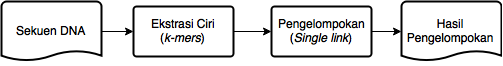
\includegraphics[width=200pt]{metode.png}
\caption{Tahapan proses penelitian}
\label{fig:tahapan}
\end{figure}

\subsection*{Penyiapan Data}

Data yang digunakan pada penelitian ini merujuk kepada penelitian \citeauthor{TAMSIN2013} (\cite*{TAMSIN2013}). Data tersebut menggunakan 50 data sekuen DNA yang terdiri dari 10 data dari genus \textit{Borellia}, 10 genus dari \textit{Streptococcus}, 10 genus dari \textit{Yersinia}, 10 genus dari \textit{Methylobacterium}, dan 10 genus dari Bacillus. Semua data diperoleh dari situs National Center of Biotechnology Information, US National Library of Medicine dalam format FASTA.

\begin{table*}[t!]
	\begin{center}
		\caption{Rencana Jadwal Penelitian}
		\label{tab:jadwal}
		\footnotesize
		\begin{tabular}{|l|c|c|c|c|c|c|c|c|c|c|c|c|c|c|c|c|c|c|c|c|}
			\hline
			\multirow{2}{*}{Kegiatan}&\multicolumn{4}{c|}{Juni}&\multicolumn{4}{c|}{Juli}&\multicolumn{4}{c|}{Agustus}&\multicolumn{4}{c|}{September}&\multicolumn{4}{c|}{Oktober}\\
			\cline{2-21}
			&1&2&3&4&1&2&3&4&1&2&3&4&1&2&3&4&1&2&3&4\\
			\hline
			Pengumpulan data dan anlisis kebutuhan sistem&\cellcolor{black}&\cellcolor{black}&\cellcolor{black}&&&&&&&&&&&&&&&&&\\
			\hline
			Perancangan dan pemodelan &&&&\cellcolor{black}&\cellcolor{black}&\cellcolor{black}&\cellcolor{black}&\cellcolor{black}&\cellcolor{black}&\cellcolor{black}&\cellcolor{black}&\cellcolor{black}&&&&&&&&\\
			\hline
			%Pemodelan data warehouse &&&&&&\cellcolor{black}&\cellcolor{black}&\cellcolor{black}&&&&&&&&&&&&\\
			%\hline
			Implementasi Sistem&&&&&&&&&\cellcolor{black}&\cellcolor{black}&\cellcolor{black}&\cellcolor{black}&&&&&&&&\\
			\hline
			Penulisan skripsi final&\cellcolor{black}&\cellcolor{black}&\cellcolor{black}&\cellcolor{black}&\cellcolor{black}&\cellcolor{black}&\cellcolor{black}&\cellcolor{black}&\cellcolor{black}&\cellcolor{black}&\cellcolor{black}&\cellcolor{black}&\cellcolor{black}&\cellcolor{black}&\cellcolor{black}&\cellcolor{black}&&&&\\
			\hline
			Seminar&&&&&&&&&&&&&&&&&\cellcolor{black}&&&\\
			\hline
		\end{tabular}
		\normalsize
	\end{center}
\end{table*}

\subsection*{Ekstraksi Ciri}
Pada tahap ini akan dilakukan ekstraksi ciri dari sekuen DNA dengan menggunakan \textit{k-mers frequency}.  Implementasi \textit{map-reduce} pada tahap ini dengan memetakan sekuen DNA ke dalam \textit{mappers}. Setiap mappers akan menghitung \textit{k-mers frequency} dari reads yang sudah dipetakan. Hasilnya akan langsung menjadi output tanpa harus melakukan \textit{reducers}. Ilustrasi proses \textit{map-reduce} untuk ekstraksi ciri dapat dilihat pada Gambar \ref{fig:kmers}.

\begin{figure}[h!]\centering % Gunakan \begin{figure*} untuk memasukkan Gambar
	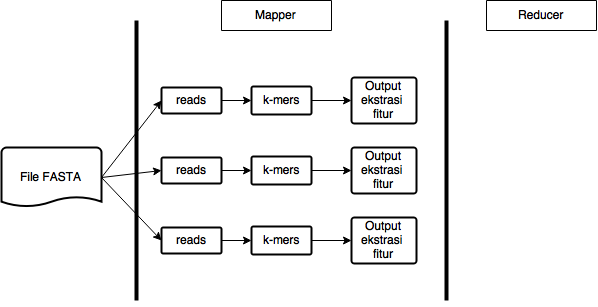
\includegraphics[width=200pt]{kmers.png}
	\caption{Illustrasi \textit{k-mers frequency} dengan model \textit{map-reduce}}
	\label{fig:kmers}
\end{figure}

\subsection*{Pengelompokan}
Ilustrasi untuk pemodelan \textit{map-reduce} dengan \textit{single link} dapat dilihat  pada Gambar \ref{fig:single}.
\begin{figure}[h!]\centering % Gunakan \begin{figure*} untuk memasukkan Gambar
	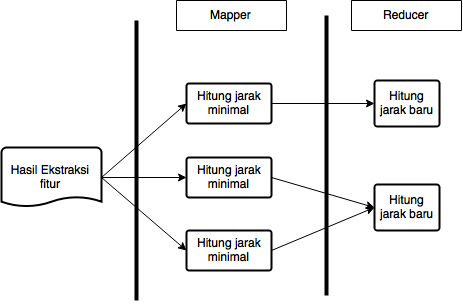
\includegraphics[width=200pt]{single.png}
	\caption{Illustrasi \textit{single link} dengan model \textit{map-reduce}}
	\label{fig:single}
\end{figure}
Ilustrasi untuk pemodelan \textit{map-reduce} dengan \textit{single link} dapat dilihat  pada Gambar \ref{fig:single}.Pada tahap ini dilakukan pengelompokan dengan menggunakan \textit{single link}. Pengelompokan dilakukan dengan data tingkat kesamaan yang didapat dari ekstraksi fitur, dimulai dengan pengelompokan menggunakan 1 data tiap genus, hingga 9 data sekuen setiap genus. Hasil dari ekstraksi akan dihitung jarak terdekatnya dan dipilih sebagai kluster, selanjutnya akan dihitung kembali jarak baru dengan memilih jarak terdekat dari kluster yang telah terpilih. 



\subsection*{Evaluasi}
Hasil dari pengelompokan \textit{single link} akan dievaluasi dengan menghitung akurasi yang diperoleh. Akurasi  akan dihitung menggunakan persamaan sebagai berikut:

\begin{equation}
Akurasi = \dfrac{\Sigma{\ data\ benar}}{\Sigma{\ jumlah\ data}}\times 100\%
\label{eq:persamaan1}
\end{equation}

\subsection*{Jadwal Kegiatan}
Penelitian ini akan dilakukan selama 4.5 bulan dengan rincian kegiatan seperti tercantum pada Tabel \ref{tab:jadwal}.



%----------------------------------------------------------------------------------------
%	BAGIAN DAFTAR PUSTAKA
%----------------------------------------------------------------------------------------

\renewcommand{\refname}{DAFTAR PUSTAKA}
\nocite{*}
\printbibliography
%----------------------------------------------------------------------------------------

\end{document}